\chapter{\OM Objects}\label{cha_obj}

In this chapter we provide a self-contained description of \OM objects. We first do so by
means of an abstract grammar description (\ref{sec_omabs}) and then give a more informal
description (\ref{sec_omin}).

\section{Formal Definition of \OM Objects}\label{sec_omabs}


\OM represents mathematical objects as terms or as labelled
trees that are called \OM objects or \OM expressions. The definition
of an abstract \OM object is then the following.



\subsection{Basic \OM objects}\label{sec_basic} 

Basic \OM Objects form the leaves of the \OM Object tree.  A Basic \OM Object is of one of
the following.
 
\begin{itemize}
\item[(i)] Integer.  Integers in the mathematical sense, with no predefined range.  They
  are \textquote{infinite precision} integers (also called \textquote{bignums} in computer
  algebra).
\item[(ii)] \acronym{ieee} floating point number.  Double precision floating-point numbers
  following the \acronym{ieee} 754-1985 standard~\cite{ieee754_85}.
\item[(iii)] Character string.  A Unicode Character string. This also corresponds to
  \textquote{characters} in \XML.
\item[(iv)] Bytearray.  A sequence of bytes.
\item[(v)] Symbol.  A Symbol encodes three fields of information, a \emph{symbol name}, a
  \emph{Content Dictionary name}, and (optionally) a \emph{Content Dictionary base URI},
  The name of a symbol is a sequence of characters matching the regular expression
  described in \ref{sec_names}.  The Content Dictionary is the location of the definition
  of the symbol, consisting of a name (a sequence of characters matching the regular
  expression described in \ref{sec_names}) and, optionally, a unique prefix called a
  \emph{cdbase} which is used to disambiguate multiple Content Dictionaries of the same
  name.  There are other properties of the symbol that are not explicit in these fields
  but whose values may be obtained by inspecting the Content Dictionary specified. These
  include the symbol definition, formal properties and examples and, optionally, a
  \emph{Role} which is a restriction on where the symbol may appear in an \OM object.  The
  possible roles are described in \ref{sec_roles}.
\item[(vi)] Variable.  A Variable must have a \emph{name} which is a sequence of
  characters matching a regular expression, as described in \ref{sec_names}.
\end{itemize}


\subsection{Derived \OM Objects}\label{sec_derived}

Derived \OM objects are currently used as a way by which non-\OM
data is embedded inside an \OM object.
A derived \OM object is built as follows: 
\begin{itemize}
\item[(i)] If $A$ is \emph{not} an \OM object, then $\foreign{A}$ is an \OM
  \emph{foreign object}.  An \OM foreign object may optionally have an \emph{encoding}
  field which describes how its contents should be interpreted.
\end{itemize}




\subsection{\OM Objects}\label{sec_compound}
  
\OM objects are built recursively as follows.
\begin{itemize}
\item[(i)] Basic \OM objects are \OM objects.
(Note that derived \OM objects are
\emph{not} \OM objects, but are used to construct \OM
objects as described below.)
\item[(ii)] If $A_1$,\ldots, $A_n$ ($n>0$) are \OM objects, then
  \[\application{A_1,\ldots,A_n}\]
  is an \OM \emph{application object}.
\item[(iii)] If $S_1$,\ldots, $S_n$ are \OM objects, and $A$ is an \OM object, and If
  $A_1$,\ldots, $A_n$ ($n>0$) are \OM objects or \OM derived objects, then
  \[\attribution{A, A_1 S_1,\ldots,A_n S_n}\]
  is an \OM \emph{attribution object}. $A$ is the object \emph{stripped of attributions}.
  If $S_1$,\ldots, $S_n$ are referred to as \emph{keys} and $A_1$,\ldots, $A_n$ as their
  associated \emph{values}.  If, after recursively applying stripping to remove
  attributions, the resulting un-attributed object is a variable, the original attributed
  object is called an \emph{attributed variable}.

\item[(iv)] If $B$ and $C$ are \OM objects, and $v_1$,\ldots, $v_n$ ($n\geq 0$) are \OM variables or attributed
  variables, then
  \[\binding{B, v_1,\ldots,v_n, C}\]
  is an \OM \emph{binding object}.

\item[(v)]  If $S$ is an \OM symbol, and $A_1$,\ldots, $A_n$ ($n\geq 0$) are \OM objects or
\OM derived objects, then
  \[\error{S, A_1,\ldots,A_n}\]
  is an \OM \emph{error object}.
\end{itemize}
\OM objects that are contstructed via rules (ii) to (v) are jointly called \emph{compound
  \OM objects}
\subsection{\OM Symbol Roles}\label{sec_roles}


We say that an \OM symbol is used to \emph{construct}
an \OM object if it is the first child of an \OM application,
binding or error object, or an even-indexed child of an \OM
attribution object (i.e. the \emph{key} in a
\emph{(key, value)} pair).
The \emph{role} of an \OM symbol is a restriction
on how it may be used to construct a compound \OM object and, in the
case of the key in an attribution object, a clarification of how that
attribution should be interpreted.  The possible roles are:
\begin{enumerate}[(\em i\rm)]
\item \emph{binder} The symbol may appear as the first child of an \OM binding object.
\item \emph{attribution} The symbol may be used as key in an \OM attribution object,
  i.e. as the first element of a (key, value) pair, or in an equivalent context (for
  example to refer to the value of an attribution).  This form of attribution may be
  ignored by an application, so should be used for information which does not change the
  meaning of the attributed \OM object.
\item \emph{semantic-attribution} This is the same as \emph{attribution} except that it
  modifies the meaning of the attributed \OM object and thus cannot be ignored by an
  application, without changing the meaning.
\item \emph{error} The symbol may appear as the first child of an \OM error object.
\item \emph{application} The symbol may appear as the first child of an \OM application
  object.
\item \emph{constant} The symbol cannot be used to construct an \OM compound object.
\end{enumerate}
A symbol cannot have more than one role and cannot be used to construct a compound \OM
object in a way which requires a different role (using the definition of construct given
earlier in this section).  This means that one cannot use a symbol which binds some
variables to construct, say, an application object.  However it does not prevent the use
of that symbol as an \emph{argument} in an application object (where by argument we mean a
child with index greater than 1).
 
If no role is indicated then the symbol can be used anywhere.  Note that this is not the
same as saying that the symbol's role is \emph{constant}.

\section{Further Description of \OM Objects}\label{sec_omin}

Informally, an \OM \emph{object} can be
viewed as a tree and is also referred to as a term.  The objects at
the leaves of \OM trees are called \emph{basic
objects}.  The basic objects supported by \OM are:
\begin{description}
\item[Integer]  Arbitrary Precision
integers.
\item[Float] \OM floats are \acronym{ieee} 754 Double precision floating-point
  numbers. Other types of floating point number may be encoded in \OM by the use of
  suitable content dictionaries.
\item[Character strings]are sequences of characters. These characters come from the
  Unicode standard~\cite{UNICODE}.
\item[Bytearrays] are sequences of bytes. There is no \textquote{byte} in \OM as an object
  of its own. However, a single byte can of course be represented by a bytearray of length
  1.  The difference between strings and bytearrays is the following: a character string
  is a sequence of bytes with a fixed interpretation (as characters, Unicode texts may
  require several bytes to code one character), whereas a bytearray is an uninterpreted
  sequence of bytes with no intrinsic meaning.  Bytearrays could be used inside \OM errors
  to provide information to, for example, a debugger; they could also contain intermediate
  results of calculations, or \textquote{handles} into computations or databases.
\item[Symbols] are uniquely defined by the Content Dictionary in which they occur and by a
  name.  The form of these definitions is explained in \ref{cha_cd}.  Each symbol has no
  more than one definition in a Content Dictionary. Many Content Dictionaries may define
  differently a symbol with the same name (e.g. the symbol \lstinline|union| is defined
  as associative-commutative set theoretic union in a Content Dictionary \lstinline|set1|
  but another Content Dictionary, \lstinline|multiset1| might define a symbol
  \lstinline|union| as the union of multi-sets).
\item[Variables] are meant to denote parameters, variables or indeterminates (such as
  bound variables of function definitions, variables in summations and integrals,
  independent variables of derivatives).
\end{description} 
Derived \OM objects are constructed from non-\OM data.  They differ from bytearrays in
that they can have any structure.  Currently there is only one way of making a derived \OM
object.

\begin{description}
\item[Foreign] is used to import a non-\OM object into an \OM attribution.  Examples of
  its use could be to annotate a formula with a visual or aural rendering, an animation,
  etc.  They may also appear in \OM error objects, for example to allow an application to
  report an error in processing such an object.
\end{description}
The four following constructs can be used to make compound \OM objects out of basic or
derived \OM objects.

\begin{description}
\item[Application] constructs an \OM object from a sequence of one or more \OM
  objects. The first child of an application is referred to as its \textquote{head} while
  the remaining objects are called its \textquote{arguments}.  An \OM application object
  can be used to convey the mathematical notion of application of a function to a set of
  arguments.  For instance, suppose that the \OM symbol $\sin$ is defined in a suitable
  Content Dictionary, then $\application{\sin,x}$ is the abstract \OM object
  corresponding to $\sin(x)$.  More generally, an \OM application object can be used as a
  constructor to convey a mathematical object built from other objects such as a
  polynomial constructed from a set of monomials.  Constructors build inhabitants of some
  symbolic type, for instance the type of rational numbers or the type of polynomials.
  The rational number, usually denoted as $\frac12$, is
  represented by the \OM application object $\application{Rational,1,2}$. The symbol
  $Rational$ must be defined, by a Content Dictionary, as a
  constructor symbol for the rational numbers.

  \begin{figure}\centering
    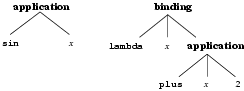
\includegraphics{lambda}
    \caption{The \OM application and binding objects for $\lambda x.x+2$ in tree-like notation.}\label{fig_obj}
  \end{figure}

\item[Binding] objects are
  constructed from an \OM object, and from a sequence of zero or more
  variables followed by another \OM object.  The first \OM object is
  the \textquote{binder} object. Arguments 2 to $n-1$ are always variables to
  be bound in the \textquote{body} which is the $n^{th}$ argument object. It
  is allowed to have no bound variables, but the binder object and the
  body should be present. Binding can be used to express functions or
  logical statements.  The function $\lambda x.x+2$, in which
  the variable $x$ is bound by $\lambda$, corresponds to a binding object having
  as binder the \OM symbol $lambda$: 
\[\binding{lambda,x,\application{plus,x,2}}\]

Phrasebooks are allowed to use $\alpha$-conversion in order to avoid clashes of
variable names. Suppose an object $\Omega$ contains an occurrence of the object
$\binding{B,v,C}$.  This object $\binding{B,v,C}$ can be replaced in $\Omega$ by
$\binding{B,z,C'}$ where $z$ is a variable not occurring free in $C$ and $C'$ is obtained
from $C$ by replacing each free (i.e., not bound by any intermediate $\mathbf{binding}$
construct) occurrence of $v$ by $z$.  This operation preserves the semantics of the object
$\Omega$. In the above example, a phrasebook is thus allowed to transform the object to,
e.g.
\[\binding{lambda,x,\application{plus,x,2}}\]


Repeated occurrences of the same variable in a binding operator
  are allowed. An \OM application should treat a binding with
  multiple occurrences of the same variable as equivalent to the
  binding in which all but the last occurrence of each variable is
  replaced by a new variable which does not occur free in the body of
  the binding.
  \[\binding{lambda,v,v,\application{times,v,v}}\]
is semantically
  equivalent to: 
  \[\binding{lambda,v',v,\application{times,v,v}}\]
  so that the resulting function is actually a constant in its first argument ($v'$ does
  not occur free in the body $\application{times,v,v}$.

\item[Attribution] decorates an object with a sequence of one or more pairs made up of an
  \OM symbol, the \textquote{attribute}, and an associated object, the \textquote{value of
    the attribute}.  The value of the attribute can be an \OM attribution object
  itself. As an example of this, consider the \OM objects representing groups,
  automorphism groups, and group dimensions. It is then possible to attribute an \OM
  object representing a group by its automorphism group, itself attributed by its
  dimension.

  \OM objects can be attributed with \OM foreign objects, which are containers for non-\OM
  structures.  For example a mathematical expression could be attributed with its spoken
  or visual rendering.



Composition of attributions, as in
\[\attribution{\attribution{A,S_1 A_1,\ldots, S_h A_h}, S_{h+1} A_{h+1},\ldots, S_n A_n}\] 
is semantically equivalent to a single attribution, that is
\[\attribution{A,S_1 A_1,\ldots, S_n A_n}\] 
The operation that produces an object with a single layer of attribution is called
\emph{flattening}.

Multiple attributes with the same name are allowed.  While the order of the given
attributes does not imply any notion of priority, potentially it could be significant. For
instance, consider the case in which $S_h=S_n$ ($h<n$) in the example above. Then, the
object is to be interpreted as if the value $A_n$ overwrites the value $A_h$.  (\OM
however does not mandate that an application preserves the attributes or their order.)


Attribution acts as either adornment annotation or as semantical annotation. When the key
has role \emph{attribution}, then replacement of the attributed object by the object
itself is not harmful and preserves the semantics. When the key has role
\emph{semantic-attribution} then the attributed object is modified by the attribution and
cannot be viewed as semantically equivalent to the stripped object. If the attribute lacks
the role specification then attribution is acting as adornment annotation.
  
Objects can be decorated in a multitude of ways.

An example of the use of an adornment attribution would be to indicate the colour in which
an \OM object should be displayed, for example $\attribution{A,colour,red}$.  Note that
both $A$ and $red$ are arbitary \OM objects whereas $color$ is a symbol.  An example of
the use of a semantic attribution would be to indicate the type of an object.  For example
the object $\attribution{A,type,t}$ represents the judgment stating that object $A$ has
type $t$. Note that both $A$ and $t$ are arbitary \OM objects whereas $type$ is a symbol.

\item[Error] is made up of an \OM symbol and a sequence of zero or more \OM objects. This
  object has no direct mathematical meaning.  Errors occur as the result of some treatment
  on an \OM object and are thus of real interest only when some sort of communication is
  taking place. Errors may occur inside other objects and also inside other errors.  Error
  objects might consist only of a symbol as in the object: $\error{S}$.
\end{description} 


\section{Names}\label{sec_names}

The names of symbols, variables and content dictionaries must conform to the production
\lstinline|Name| specified in the following grammar (which is identical to that for \XML
names in XML 1.1, \cite{xml_04}). Informally speaking, a name is a sequence of Unicode
\cite{UNICODE} characters which begins with a letter and cannot contain certain
punctuation and combining characters.  The notation \lstinline|#x...| represents the
hexadecimal value of the encoding of a Unicode character.  Some of the character values or
\emph{code points} in the following productions are currently unassigned, but this is
likely to change in the future as Unicode evolves \footnote{\label{xml1} We note that in
  XML 1 the name production explicitly listed the characters that were allowed, so all the
  characters added in versions of Unicode after 2.0 (which amounted to tens of thousands
  of characters) were not allowed in names.}


\begin{center}
\begin{tabular}{l@{$\longrightarrow$}p{10cm}}
Name & NameStartChar (NameChar)* \\
NameStartChar & 
\lstinline? ":" | [A-Z] | "_" | [a-z] | [#xC0-#xD6] | [#xD8-#xF6] |?\\
& \lstinline?[#xF8-#x2FF] | [#x370-#x37D] | [#x37F-#x1FFF] |?\\
& \lstinline?[#x200C-#x200D] | [#x2070-#x218F] | [#x2C00-#x2FEF] |?\\
& \lstinline?[#x3001-#xD7FF] | [#xF900-#xFDCF] | [#xFDF0-#xFFFD] |?\\
& \lstinline?[#x10000-#xEFFFF]? \\
NameChar & 
NameStartChar \lstinline?| "-" | "." | [0-9] | #xB7 | [#x0300-#x036F] |?\\
 & \lstinline?[#x203F-#x2040]? 
\end{tabular}
\end{center}

\paragraph{CD Base}

A cdbase must conform to the grammar for URIs described in
\cite{IETF2396}.  Note that if non-ASCII characters are
used in a CD or symbol name then when a URI for that symbol is
constructed it will be necessary to map the non-ASCII characters to a
sequence of octets.  The precise mechanism for doing this depends on
the URI scheme.


\paragraph{Note on content dictionary names}

It is a common convention to store a Content Dictionary in a file of
the same name, which can cause difficulties on many file systems.  If
this convention is to be followed then \OM
\emph{recommends} that the name be restricted to the
subset of the above grammar which is a legal POSIX
\cite{POSIX} filename, namely:

\begin{center}
\begin{tabular}{l@{$\longrightarrow$}p{10cm}}
Name & (PosixLetter \lstinline?| '_'?) (Char)*\\
Char &  PosixLetter \lstinline?| Digit | '.' | '-' | '_' ?\\
PosixLetter & \lstinline? 'a' | 'b' | ... | 'z' | 'A' | 'B' | ... | 'Z'?
\end{tabular}
\end{center}


\paragraph{Canonical URIs for Symbols}

To facilitate the use of \OM within a URI-based framework (such as RDF
\cite{rdf} or OWL \cite{owl}), we provide the
following scheme for constructing a canonical URI
for an \OM Symbol:
\begin{lstlisting}
URI = cdbase-value + '/' + cd-value + '#' + name-value
\end{lstlisting}
So for example the URI for the symbol with cdbase \url{http://www.openmath.org/cd}, cd
\lstinline|transc1| and name \lstinline|sin| is:
\begin{lstlisting}
http://www.openmath.org/cd/transc1#sin
\end{lstlisting}
In particular, this now allows us to refer uniquely to an \OM symbol from a
MathML document \cite{MathML_2003}:
\begin{lstlisting}
<mathml:csymbol xmlns:mathml="http://www.w3.org/1998/Math/MathML/"
                definitionURL="http://www.openmath.org/cd/transc1#sin">
  <mo> sin </mo> 
</csymbol>
\end{lstlisting}



\section{Summary}\label{sec_summary}

\begin{itemize}
\item \OM supports basic objects like integers, symbols, floating-point numbers, character
  strings, bytearrays, and variables.
\item \OM compound objects are of four kinds: applications, bindings, errors, and
  attributions.
\item \OM objects may be attributed with non-\OM objects via the use of foreign \OM
  objects.
\item \OM objects have the expressive power to cover all areas of computational
  mathematics.
\end{itemize}

Observe that an \OM application object is viewed as a \textquote{tree} by software
applications that do not understand Content Dictionaries, whereas a Phrasebook that
understands the semantics of the symbols, as defined in the Content Dictionaries, should
interpret the object as functional application, constructor, or binding accordingly. Thus,
for example, for some applications, the \OM object corresponding to $2+5$ may result in a
command that writes $7$.



%%% Local Variables:
%%% mode: latex
%%% TeX-master: "omstd20"
%%% End:
